\documentclass[11pt, a4paper]{article}

\usepackage{amsmath}
\usepackage{amssymb}
\usepackage{graphicx}
\usepackage{booktabs}
\usepackage{hyperref}
\usepackage{comment}
\usepackage{subcaption}
\usepackage{listings}
\usepackage{verbatim}
%\setlength{\intextsep}{12pt}      % Space 
%\setlength{\columnsep}{45pt} 
% Margins
\usepackage[top=2.5cm, bottom=2.5cm, left=2.5cm, right=2.5cm]{geometry}

% New commands for tool names
\newcommand{\ape}{\textit{ape}}
\newcommand{\dendropy}{\textit{DendroPy}}
\newcommand{\cogent}{\textit{cogent3}}
\newcommand{\biopython}{\textit{Biopython}}
\newcommand{\ete}{\textit{ete3}}
\newcommand{\toytree}{\textit{toytree}}
\newcommand{\phylo}{\textit{Phylo.jl}}
\newcommand{\gotree}{\textit{gotree}}
\newcommand{\phylors}{\textit{phylo-rs}}
\newcommand{\castor}{\textit{castor}}
\newcommand{\stan}{\textit{Stan}}
\newcommand{\turing}{\textit{Turing.jl}}
\newcommand{\biomc}{\textit{BIOMEC}}

\title{A Comparative Analysis of Phylogenetic Tree Manipulation Tools: \\
Benchmarking Tree Traversal and Coalescent Likelihood Evaluation}

\author{Emma Gairaud Hess}

\date{\today}

\begin{document}

\maketitle

% ==========================================
% ABSTRACT
% ==========================================
\begin{abstract}

Phylogenetic tree manipulation is essential in many fields of modern biology. The rise of genomic sequencing means that phylogenetic reconstruction often comprise thousands of samples, posing challenges to inference methods, which require traversing phylogenetic trees for a range of calculations. This study presents a survey and benchmarking of eight phylogenetic packages and tools,
evaluating their performance on tree traversal operations (pre-order, post-order, level-order) and ultrametricity testing.
The tests were conducted on randomly generated trees of 1{,}000 leaves.
Performance metrics were measured in a range of scripting languages: R-based (\ape, \castor), Python-based
(\dendropy, \cogent, \biopython, \ete, \toytree) and Julia-based (\phylo) tools.
Subsequently, the best-performing tools were selected, and  a coalescent likelihood evaluation framework was implemented, deriving the full log-likelihood under an exponential-growth demographic model, which is particularly relevant for phylogenetic analyses of infectious pathogens.
The modular benchmarking design allows extension to other demographic models, tree representations, and tools, with applications in epidemic outbreak modeling and parameter estimation using modern inference frameworks in general probabilistic toolkits.

\vspace{0.3cm}
\noindent \textbf{Keywords:} phylogenetics, benchmarking, tree traversal, coalescent likelihood, outbreak modeling.

\end{abstract}

\newpage
\tableofcontents
\newpage

% ==========================================
% 1. INTRODUCTION
% ==========================================
\section{Introduction}

Phylogenetic trees are fundamental data structures in biology, representing the evolutionary relationships among taxa or individuals. Although their original use was limited to describing how species are related in a taxonomic context, molecular phylogenetics goes beyond the species level and also can also include pathogens, genes and cells. It has subsequently made the same concepts relevant in fields that require the comparison of molecular sequences to infer evolutionary relationships, notably epidemiology and genomics \cite{yang2012molecular,whelan2001molecular}. 
Modern phylogenetic studies frequently involve large trees (thousands to millions of leaves \cite{ferreira2021covizu}), whose manipulation requires efficient algorithms.

Coalescent processes are used in epidemiology to provide a framework for estimating parameters such as transmission rates and the number of unsampled individuals during disease outbreaks \cite{volz2009,pybus2001}. These models require extensive tree traversal and statistical inference, making computational efficiency crucial.

Current phylogenetic software is highly diverse, with implementations available across multiple programming languages. For example, BEASTX and BEAST2 \cite{drummond2007beast, bouckaert2019beast2} use Java, but model implementation is restrictive in that they do not have the flexibility of general purpose programming languages, such as Stan (command-line, R, Python) \cite{carpenter2017stan}, Turing (Julia) \cite{ge2018turing}, or PyMC (Python) \cite{salvatier2016pymc}.

Comparing packages across languages highlights the different trade-offs between development speed, execution speed and ecosystem diversity. R is essential for statistical phylogenetics, Python offers a plethora of bioinformatic tools, and, although it is less developed, Julia theoretically offers both high-level syntax and low-level fast compilation \cite{bezanson2017julia}. Understanding how the language choice affects real running time operations is key when selecting software for larger analytical frameworks. 

Tree traversal is not merely a low-level routine; it underpins almost every higher-level phylogenetic computation. Likelihood calculation, for example, typically requires one or more post-order traversals to propagate partial likelihoods from tips to root \cite{felsenstein1981evolutionary}. Similarly, operations such as subtree extraction, node-depth computation, and tree distance metrics all depend on efficient and repeated traversal of the tree structure. Therefore, the cost of traversal sets an upper bound on the practical scalability of these downstream methods. 

While other studies focus on phylogenetic inference accuracy \cite{hoehler2025phylosmew}, comparative performance evaluation of fundamental tree operations is limited.

This report addresses two main objectives. Firstly, benchmarking basic tree operations across several phylogenetic packages and to establish their relative efficiency. This acts as a filter, where only the best performing and more relevant tools are kept. These are then used on the second objective of the study: after establishing a computational framework for coalescent likelihood evaluation, its efficiency is also evaluated among the chosen tools. 
It also lays the foundation for future work on more complex models and on implementing ways to improve their efficiency. This can then be integrated into a bigger workflow that returns parameter estimations through a variety Monte-Carlo Markov Chain (MCMC) algorithms used in Bayesian Inference.

% ==========================================
% 2. METHODS
% ==========================================
\section{Methods}

% ------------------------------------------
\subsection{Part I: Tree Traversal Benchmarking}
% ------------------------------------------

\subsubsection{Traversal strategies}

A standardized benchmarking framework was implemented to evaluate four core operations for tree manipulation:
\begin{itemize}
    \item \textbf{Pre-order traversal:} Root-to-leaf depth-first search (DFS) (fig.\ref{fig:tree_traversals}-A)
    \item \textbf{Post-order traversal:} Leaf-to-root DFS (fig.\ref{fig:tree_traversals}-B)
    \item \textbf{Level-order traversal:} Queue-based breadth-first search (BFS) (fig.\ref{fig:tree_traversals}-C)
    \item \textbf{Ultrametricity evaluation:} Verifies that all leaves are equidistant from the root (fig.\ref{fig:tree_ult}). It serves as a manual test for most tools, since only \ape\ contains a native method for this. It is also a full tree traversal in practice when used on ultrametric trees. 
\end{itemize}

\begin{figure}[htbp]
    \centering
    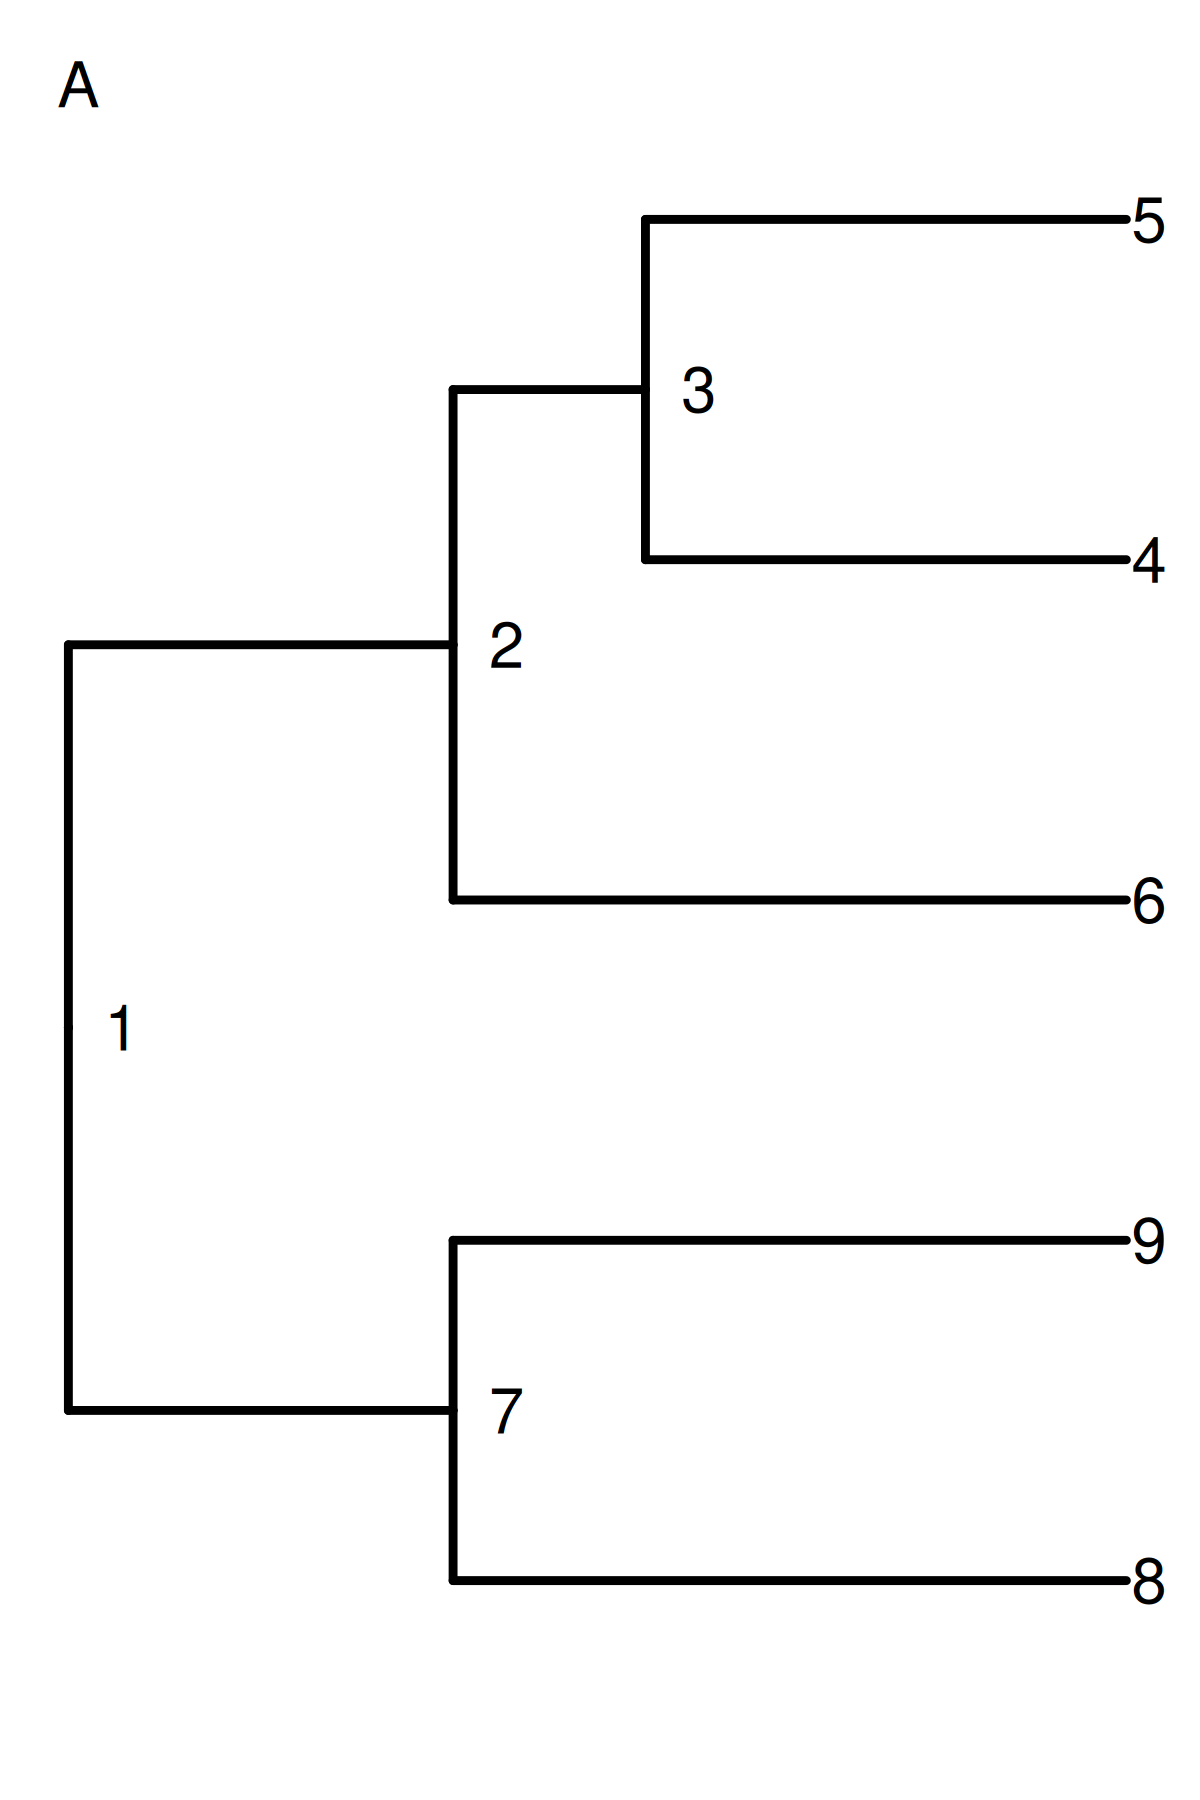
\includegraphics[width=0.3\textwidth]{preordervf.png}
    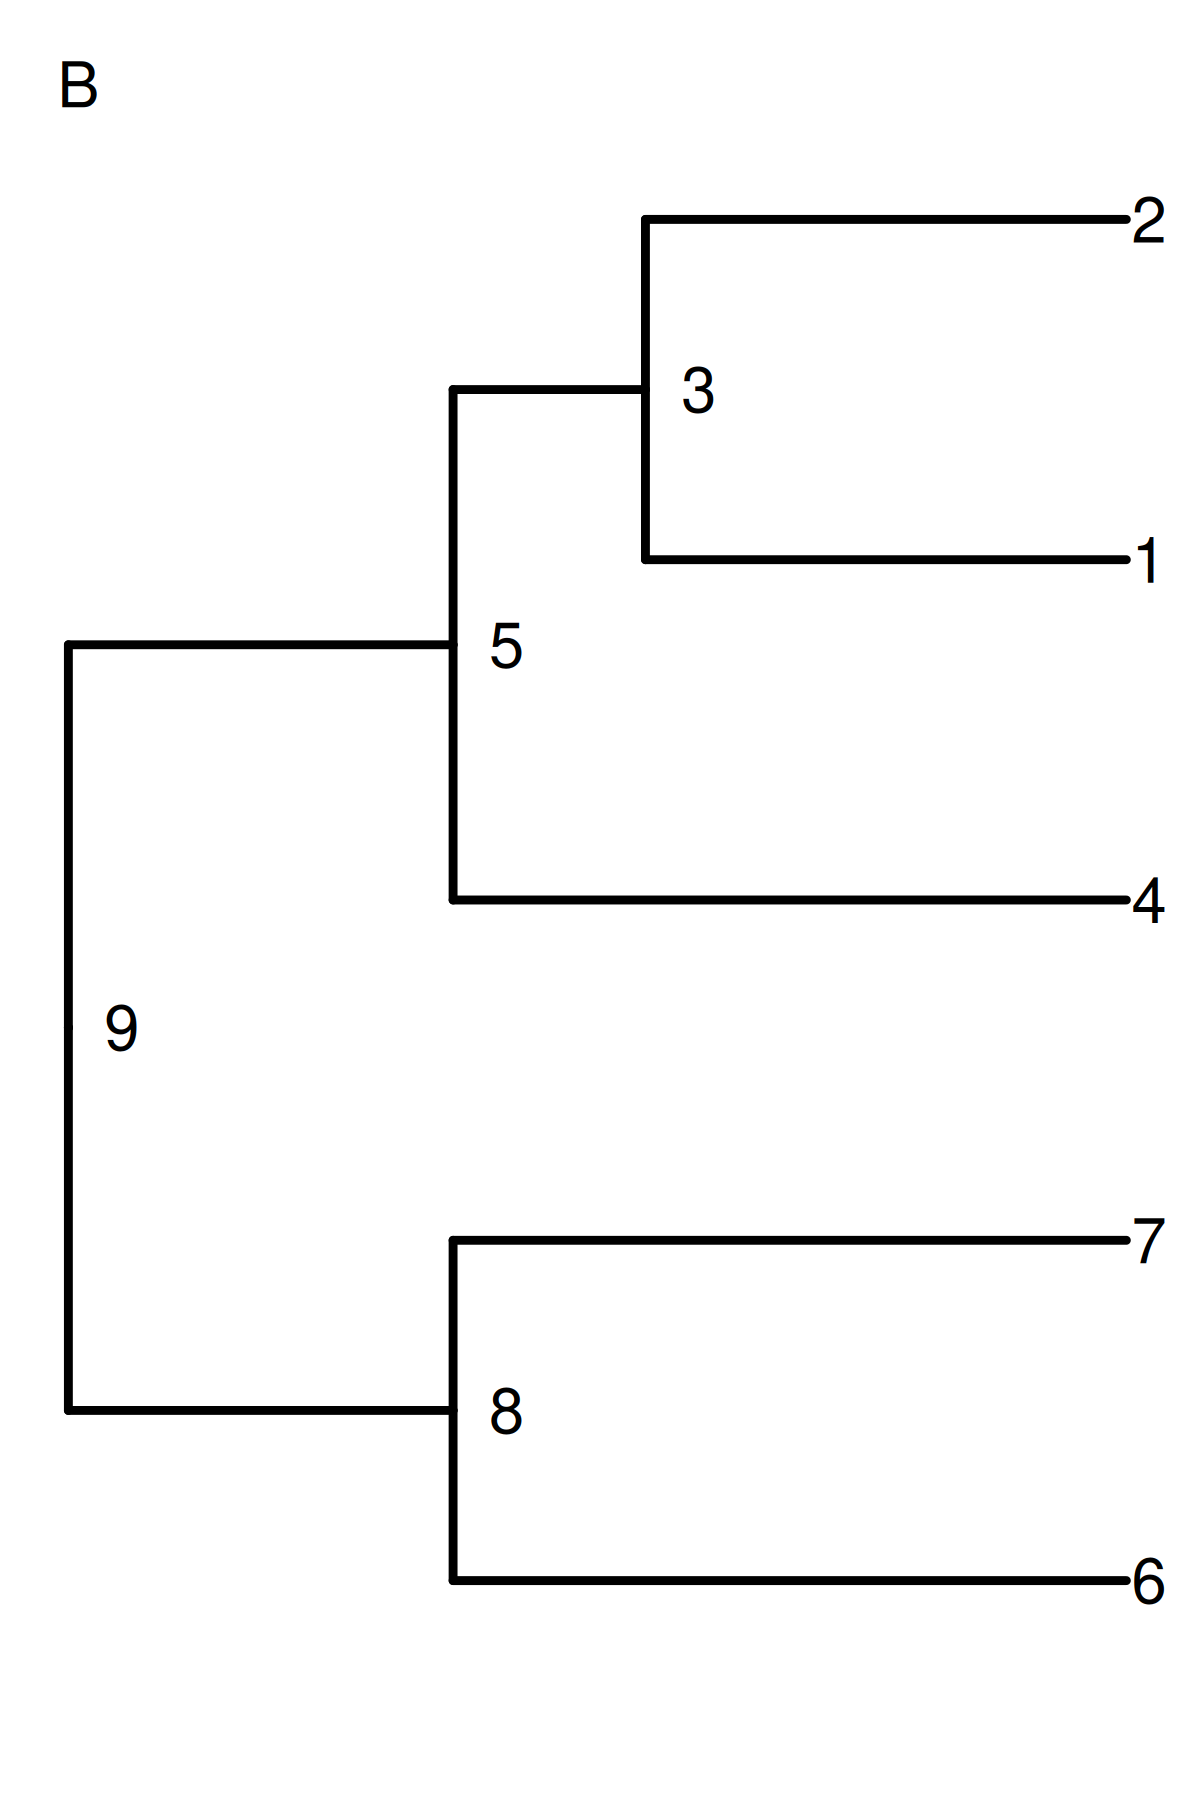
\includegraphics[width=0.3\textwidth]{postordervf.png}
    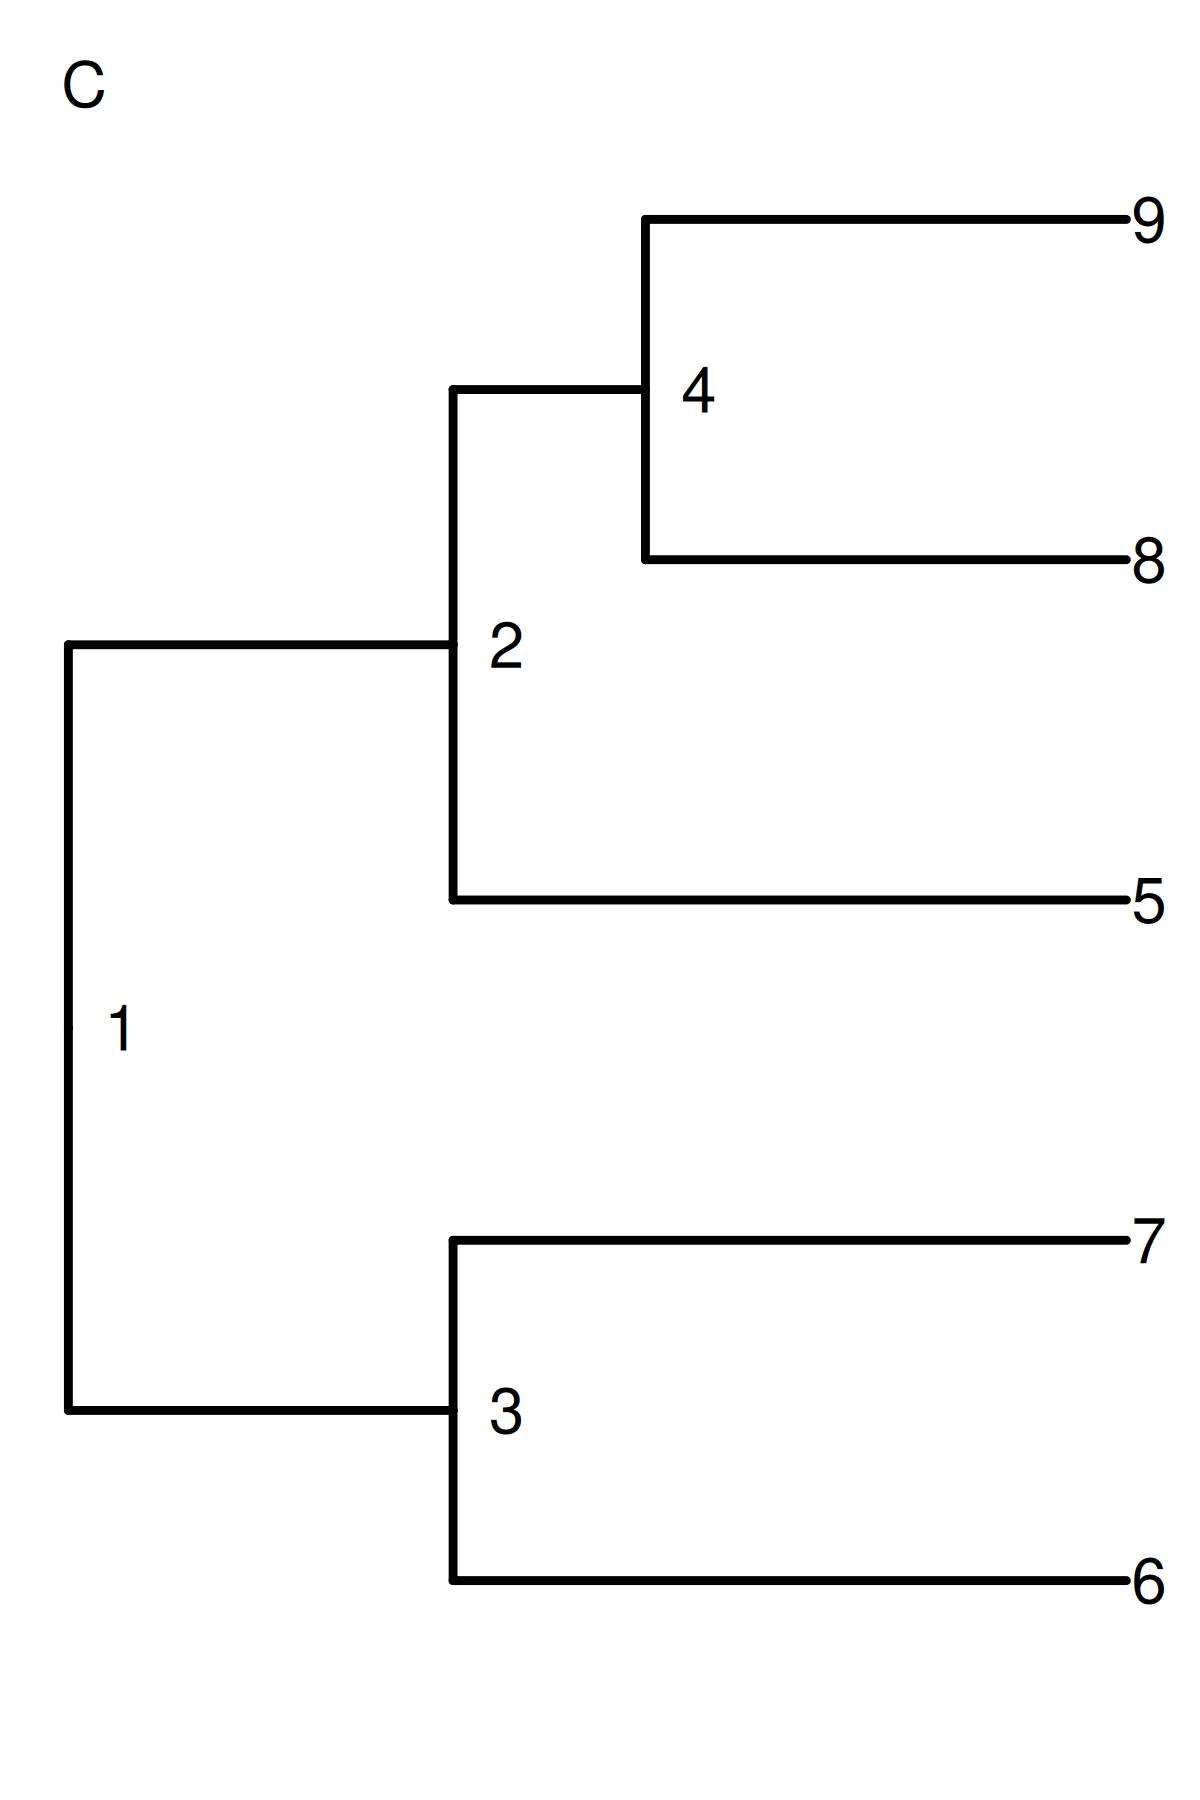
\includegraphics[width=0.3\textwidth]{levelordervf.png}
    \caption{Pre-order (A), post-order (B) and level-order (C) traversal on the same tree; each number corresponds to the order in which the nodes are visited.}
    \label{fig:tree_traversals}
\end{figure}

\subsubsection{Tree Generation}

To make fair comparisons across all tests, it was necessary to generate a dataset compatible with every tool. Test trees with 1{,}000 leaves each were generated in \ape\ with a set seed, by using the following built-in functions:
\begin{itemize}
    \item \textbf{rcoal(n)}: generates a coalescent (specific type of ultrametric) tree of $n$ leaves by randomly clustering its tips; it was used for the ultrametric tree set
    \item \textbf{rtree(n)}: generates a general tree of $n$ leaves by randomly splitting its edges; the heterochronic (non-ultrametric) tree set was made with it 
\end{itemize}

For each tree type, 1{,}000 trees were generated and stored in \texttt{.nwk} format files, which is compatible with all the tested phylogenetic tools. 

\begin{figure}
    \centering
    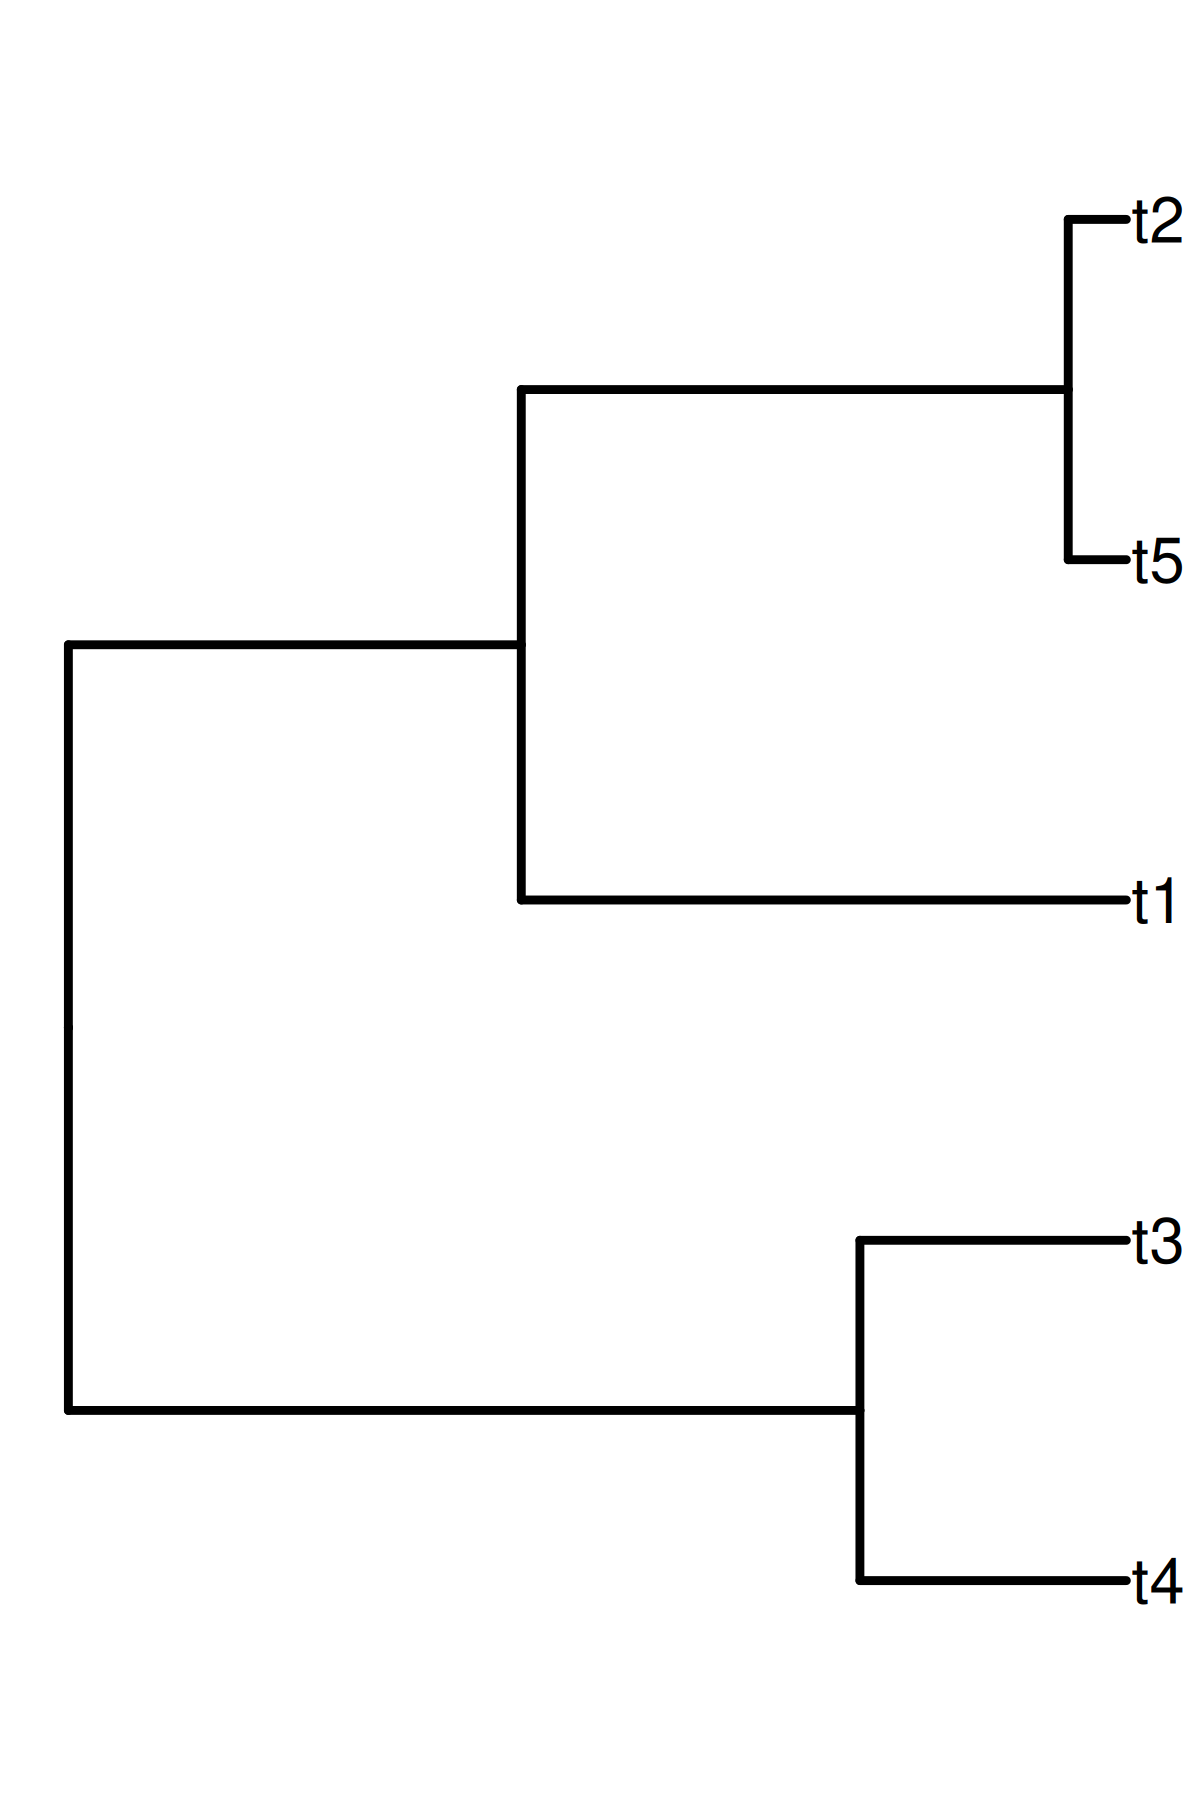
\includegraphics[width=0.35\textwidth]{coalescentr.png}
    \hspace{0.1\textwidth}
    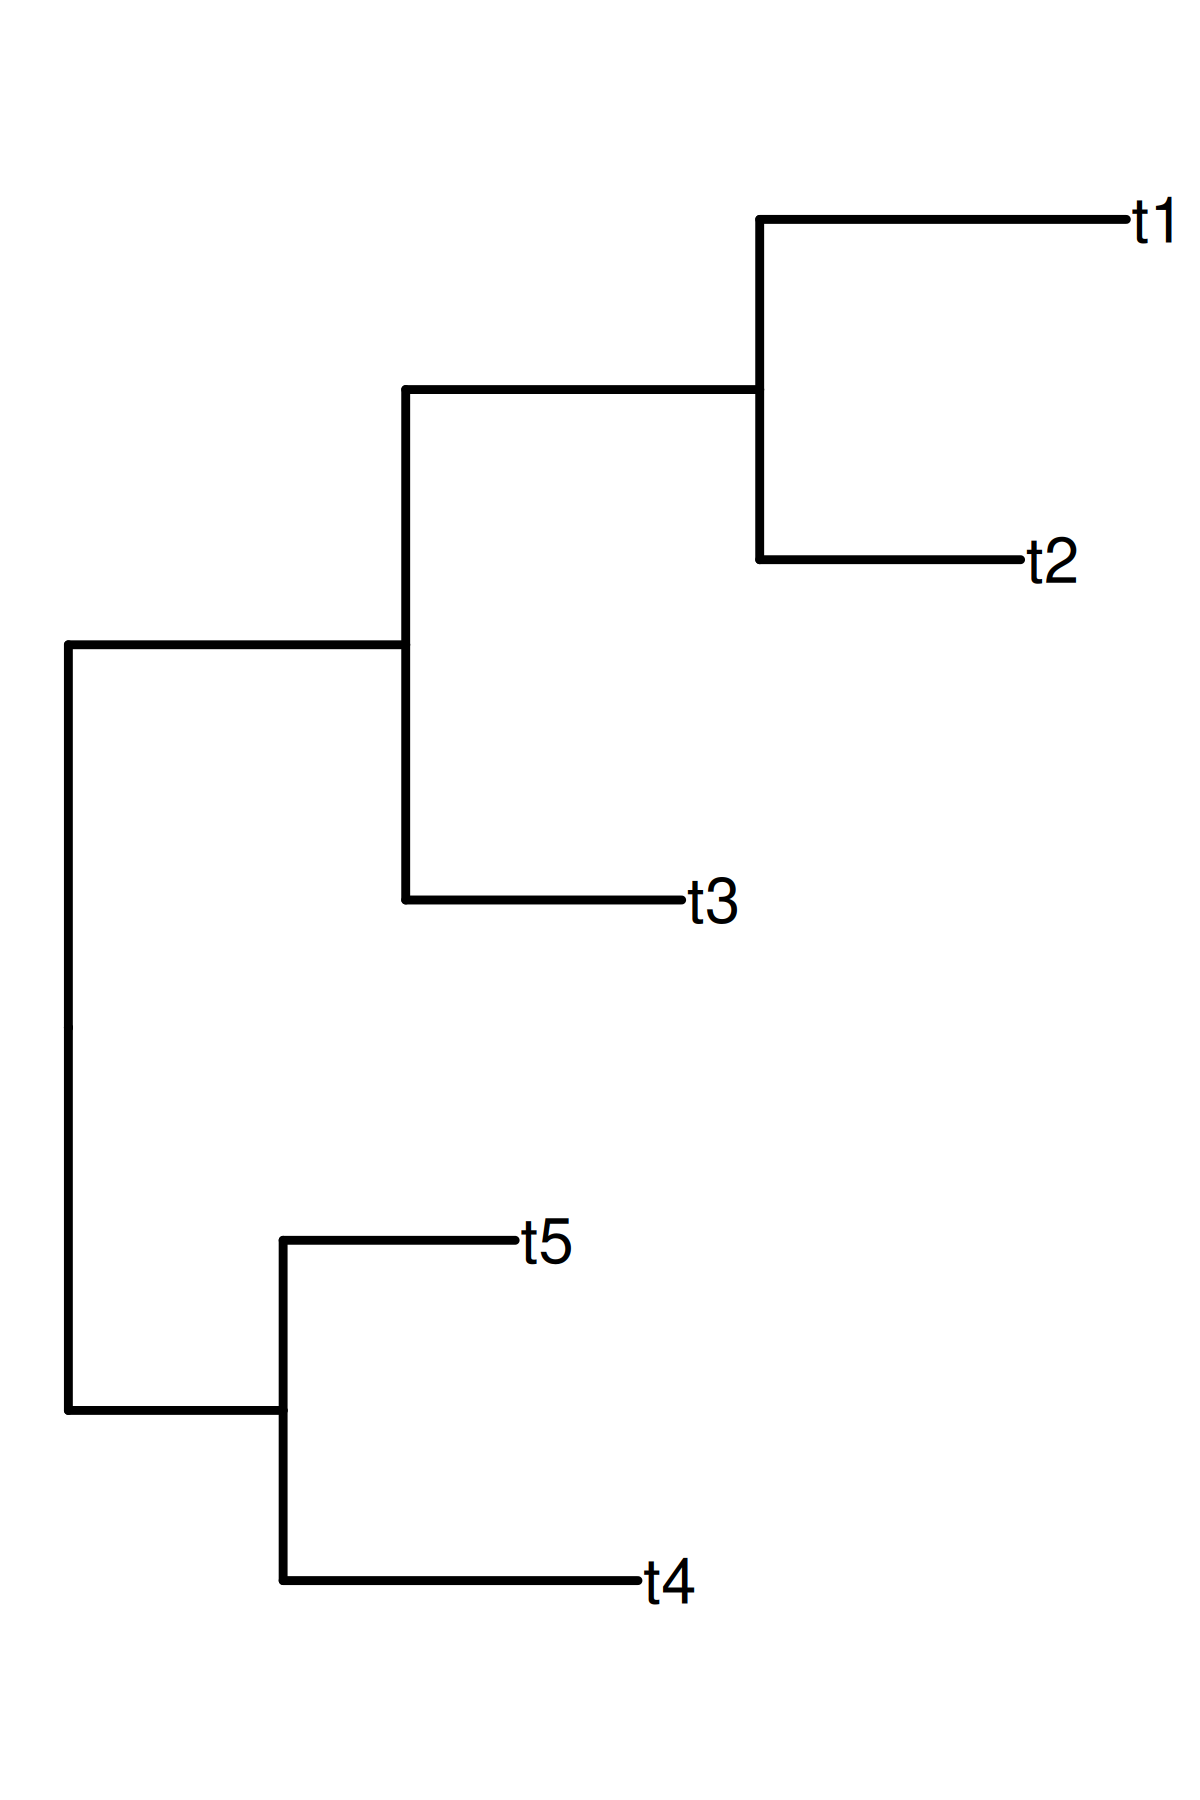
\includegraphics[width=0.35\textwidth]{heterochronictr.png}
    \caption{An illustration of an ultrametric (left) and a heterochronic (right) tree}
    \label{fig:tree_ult}
\end{figure}

\subsubsection{Benchmarking Procedure}

Timing measurements were done after a warmup iteration to account for just-in-time compilation (JIT) and memory allocation (e.g. garbage collection - GC). Execution times were recorded using system timers (\texttt{Sys.time()} for R, \texttt{time.perf\_counter()} for Python and \texttt{time\_ns()} for Julia) to calculate the time it takes $t_{taken}$ to perform a given function $fn$: 

\begin{align*}
    t_{start} &= \text{system\_timer} \\
    fn \\
    t_{end} &= \text{system\_timer} \\
    t_{taken} &= t_{end} - t_{start}
\end{align*}

$t_{taken}$ is then converted into microseconds.

As the tests would have to be done on 1000 trees, a for loop was added. On each tool, the same method was used to benchmark both the tree traversal and coalescent likelihood methods. 

\subsubsection{Tools Evaluated}

\paragraph{\ape} (R package)

An R package for phylogenetic analysis. It stores trees as edge lists matrices in R and improves the performance of certain operations (e.g. reordering, node-depth calculation) by compiling in C/C++ code \cite{paradis2004ape}.Benchmarks use the package's \texttt{is.ultrametric()} function for ultrametricity evaluation, as well as a manual implementation of the three traversal strategies.

\paragraph{\castor} (R package)

Specialized R package for large-scale tree inference and analysis, \castor\ stores trees using the same \ape-compatible \texttt{phylo} objects, while adding additional routines for ancestral state reconstruction and diversification modeling \cite{teufel2018castor}. Some of its functions are compiled in C/C++. While \texttt{get\_all\_distances\_to\_root()} is a built-in distance computation that uses level-order traversal, all core operations for the study were implemented manually.  

\paragraph{\dendropy} (Python)

Python implementation of phylogenetic data structures.\dendropy\ uses object-oriented design with \texttt{Node} and \texttt{Tree} classes \cite{sukumaran2010dendropy}. It has no compiled backend, so performance can be bottle-necked by the Python interpreter overhead \cite{berger2022scalene}. Iterators for all three traversal methods exist for tree objects (\texttt{tree.preorder\_node\_iter()},\texttt{tree.postorder\_node\_iter()}, \\ \texttt{tree.levelorder\_node\_iter()}), and the ultrametricity check was implemented manually. 

\paragraph{\cogent} (Python)

The modern, python-3 compatible successor of \textit{PyCogent}, \cogent\ provides phylogenetic data structures in Python and uses NumPy for array-based operations; some of its functions are Cython-accelerated, but tree traversal remains predominantly Python \cite{cogent32024,knight2007pycogent}. Native methods \texttt{tree.preorder()}, \texttt{tree.postorder()} and \texttt{tree.levelorder()}, as well as a manual ultrametricity evaluator were used. 

\paragraph{\biopython} (Python)

A general-purpose bioinformatics package with a phylogenetic submodule (\textit{Bio.Phylo}). Provides wrappers around external phylogenetic tools while offering native Python tree structures \cite{cock2009biopython} and emphasizes compatibility over computational efficiency. For each strategy, \\\texttt{tree.find\_elements(target=TreeElement, order=strategy)} was used, and the ultrametricity evaluation was coded manually. 

\paragraph{\ete} (Python)

A pure Python library focused on interactive phylogenetic analysis, visualization and tree annotation \cite{huerta2016ete3}. It has no compiled backend. The method \texttt{tree.traverse(strategy)} was used for simple traversals and ultrametricity evaluation was manually implemented. 

\paragraph{\toytree} (Python)

Built on \textit{toyplot}, \toytree\ is a lightweight Python tree library for phylogenetics that uses simple array-based tree representations. It can be integrated into Jupyter notebooks and has no compiled backend \cite{eaton2020toytree}. Its traversal syntax is identical to \ete's (\texttt{tree.traverse(strategy)}) and it also has a manually implemented ultrametricity evaluation. 

\paragraph{\phylo} (Julia)

A Julia package providing multiple-dispatch tree implementations \cite{phylojl2024}. Julia's multiple dispatch and LLVM-based JIT compilation should enable performances comparable to C \cite{bezanson2017julia}. \phylo has a built-in traversal method as well: \texttt{traversal(tree,strategy)} but no native ultrametricity evaluator. 

\subsubsection{Statistical Analysis}

For each tool and operation, summary statistics were computed: mean, median, and standard deviation of execution times give us an idea of the overall efficiency of a tool, while minimum and maximum time values help to identify outliers in the data or implementation.  

Summary visualizations (violin plots) were generated for qualitative comparison.

Tools presenting outlier max values had a max index tracker to verify the source of the problem.

A bash file was made to run the scripts for the selected tools, append the test results to an output file, and store the output file and images in a distinct directory was made to keep track of the different results over time.

% ------------------------------------------
\subsection{Part II: Coalescent Likelihood Framework}
% ------------------------------------------

\subsubsection{Biological Motivation}

Kingman's $n$-coalescent is a stochastic process that describes the genealogical ancestry of a random sample of $n$ individuals drawn from a large population assuming exchangeable reproduction, going backwards in time \cite{kingman1982}. It is the mathematical foundation for likelihood-based inference of effective population size $N_e$ from phylogenetic trees, and is closely related to birth-death models used in epidemiology and other fields.

\subsubsection{Kingman's Coalescent Process}

Consider a sample of $n$ lineages observed at time $t = 0$ and going backwards in time. Under the standard Wright-Fisher model with effective population size $N_e$, the probability that any specific pair of lineages coalesces in the previous generation
is $1/N_e$. The waiting time until the first coalescence event among $k$ extant lineages follows an
exponential distribution.

\medskip
\noindent\textbf{Coalescence rate.}
When $k$ lineages are present, there are $\binom{k}{2} = k(k-1)/2$ distinct pairs,
each coalescing at rate $1/N_e$, giving a total instantaneous coalescence rate of: 

\begin{equation}
    \gamma_k = \frac{\binom{k}{2}}{N_e} = \frac{k(k-1)}{2N_e}.
    \label{eq:coalrate}
\end{equation}

\noindent\textbf{Waiting time distribution.}
Denoting the waiting time during which exactly $k$ lineages are present as $w_k$,
we have
\begin{equation}
    w_k \sim \mathrm{Exp}\!\left(\gamma_k\right),
    \qquad
    f(w_k) = \gamma_k\, e^{-\gamma_k w_k},
    \quad w_k \geq 0.
    \label{eq:waitingtime}
\end{equation}

Starting with $n$ lineages, the process generates $n - 1$ coalescent events, reducing
the number of lineages from $n$ down to $1$ (the most recent common ancestor, MRCA).
The topology of which two lineages merge at each event is chosen uniformly at random
from the $\binom{k}{2}$ possible pairs.

\subsubsection{Coalescent Likelihood Under Constant Population Size}

Let $\mathcal{T}$ denote a fully resolved rooted binary tree with $n$ leaves and
coalescent waiting times $w_n, w_{n-1}, \ldots, w_2$, where $w_k$ is the duration
during which $k$ lineages coexist (measured backwards from the sampling time).
Assuming a constant effective population size $N_e$, the likelihood of the tree
given $N_e$ factorises over coalescent intervals:

\begin{equation}
    \mathcal{L}(N_e \mid \mathcal{T})
    = \prod_{k=2}^{n}
      \frac{\binom{k}{2}}{N_e}\,
      \exp\!\left(-\frac{\binom{k}{2}}{N_e}\,w_k\right).
    \label{eq:coallikelihood}
\end{equation}

Taking logarithms yields the log-likelihood

\begin{equation}
    \ell(N_e \mid \mathcal{T})
    = \sum_{k=2}^{n}\left[\log\binom{k}{2} - \log N_e
      - \frac{\binom{k}{2}}{N_e}\,w_k\right]
    = (n-1)\bigl(-\log N_e\bigr) + C - \frac{S}{N_e},
    \label{eq:loglik}
\end{equation}

where $C = \sum_{k=2}^{n}\log\binom{k}{2}$ is a constant independent of $N_e$, and

\begin{equation}
    S = \sum_{k=2}^{n} \binom{k}{2}\,w_k
    \label{eq:sstat}
\end{equation}

is the sufficient statistic for $N_e$: the total coalescent-weighted tree length.

\medskip
\begin{comment}
\noindent\textbf{Maximum likelihood estimator(MLE).}
Setting $\partial\ell/\partial N_e = 0$ gives the closed-form MLE

\begin{equation}
    \hat{N}_e = \frac{S}{n-1}
              = \frac{1}{n-1}\sum_{k=2}^{n}\binom{k}{2}\,w_k.
    \label{eq:MLE}
\end{equation}

This estimator has an intuitive interpretation: $\hat{N}_e$ is the average
coalescent-pair--weighted waiting time per coalescent event.

In this work, $N_e$ was not estimated directly. Instead, we parametrise the coalescent rate as a function in time ($\lambda (t)$) and evaluate the log likelihood for fixed parameters. 

\subsubsection{Extension to Variable Effective Population Size}

In practice, $N_e$ may change over time, for example due to population expansions or epidemic dynamics. Griffiths and Tavaré (1994) \cite{griffiths1994} generalized the
coalescent to allow a time-varying effective population size $N_e(t)$, where $t$
increases into the past from the sampling time $t = 0$.

\medskip
\noindent\textbf{Likelihood with $N_e(t)$.}
When $k$ lineages are present starting at backward time $t_k$, the probability density
of the waiting time $w_k$ is

\begin{equation}
    f\!\left(w_k \mid t_k,\, N_e(\cdot)\right)
    = \frac{\binom{k}{2}}{N_e(t_k + w_k)}\,
      \exp\!\left(-\binom{k}{2}\int_{t_k}^{t_k + w_k}
      \frac{dt}{N_e(t)}\right),
    \label{eq:varcoal}
\end{equation}

and the full log-likelihood is obtained by summing the logarithms of
Eq.~\eqref{eq:varcoal} over all $n-1$ coalescent intervals.

\medskip
\noindent\textbf{Constant-size case.}
Under a constant-size model, $N_e(t) = N_e$ for all $t$, and
Eq.~\eqref{eq:varcoal} reduces to the exponential waiting-time distribution in
Eq.~\eqref{eq:waitingtime}. Given a set of coalescent intervals, one can write the
likelihood as a function of $N_e$ and find the maximum-likelihood estimate by
differentiating the log-likelihood with respect to $N_e$ and setting the derivative
to zero.

\begin{equation}
    N_e(t) = \theta_j \quad \text{for } t \in [x_{j-1},\, x_j),
    \quad j = 1, \ldots, M+1.
    \label{eq:piecewise}
\end{equation}

Within each grid interval, the integral in Eq.~\eqref{eq:varcoal} reduces to a sum of
terms of the form $\binom{k}{2}\,\Delta t / \theta_j$, recovering the constant-$N_e$
structure and enabling efficient recursive computation during tree traversal.

The joint log-likelihood over all intervals and all $n-1$ coalescent events is:

\begin{equation}
    \ell\!\left(\boldsymbol{\theta} \mid \mathcal{T}\right)
    = \sum_{j=1}^{M+1}\left[-c_j\log\theta_j - \frac{\mathrm{SS}_j}{\theta_j}\right]
    + \text{const},
    \label{eq:pccoal}
\end{equation}

where $c_j$ is the number of coalescent events in interval $j$, and
$\mathrm{SS}_j = \sum_k \binom{k}{2}\,\Delta t_{k,j}$ accumulates the
coalescent-pair--weighted duration of all lineage intervals that overlap grid cell $j$.
\end{comment}

\subsubsection{Exponential-Growth Coalescent Model}

In real world applications, $N_e$ is rarely constant through time. A common model used for variable size is the exponential-growth coalescent, in which the population size grows or declines exponentially from the present and into the past \cite{drummond2002}: 

\begin{equation}
N_e(t) = \phi_0\,e^{-rt},
\label{eq:exp_ne}
\end{equation}

where $t$ is time before present, $\phi_0=N_e(0)$ is the effective population size at present, and $r$ is the exponential growth rate. The corresponding coalescent rate while $k$ lineages are active is:

\begin{equation}
\lambda_k(t) = \frac{\binom{k}{2}}{N_e(t)}
             = \binom{k}{2}\frac{e^{rt}}{\phi_0}.
\label{eq:exp_rate}
\end{equation}

When \(N_e\) is constant (\(r=0\)), the waiting time until the next coalescence is simply exponential, as in Eq.~\eqref{eq:waitingtime}. Under exponential growth, the waiting-time density starting at backward time $t_k$ is generalized to

\begin{equation}
f(w_k\mid t_k,\phi_0,r)
=
\binom{k}{2}\frac{e^{r(t_k+w_k)}}{\phi_0}
\exp\!\left[
-\frac{\binom{k}{2}}{\phi_0}\,
\frac{e^{r(t_k+w_k)}-e^{rt_k}}{r}
\right],
\quad w_k\ge 0.
\label{eq:exp_wait}
\end{equation}

Equation~\eqref{eq:exp_wait} reduces to the constant-size exponential density when \(r\to 0\). For serially sampled trees, the genealogy is partitioned into intervals \([a_i,b_i]\) with constant lineage counts \(k_i\); each interval contributes a survival factor from the exponential in Eq.~\eqref{eq:exp_wait}, and intervals ending in a coalescent event contribute the instantaneous rate \(\lambda_{k_i}(b_i)\). This yields the log-likelihood used in the implementation below.

This equation gives interval-specific contributions used in our implementation by making serial sampling simpler to incorporate, since it treats sample times as events that change $k$.

\subsubsection{Code Implementation}
For benchmarking across the different tools, we adopted the epidemiological model in which the coalescent rate $\lambda_k$ grows exponentially into the past (Eq. \ref{eq:exp_rate}).

Since the coalescent likelihood framework would be tested on heterochronic trees, which contain samples from different dates, serial sampling was used \cite{drummond2002}. 

Events are sorted by their time before present, the active lineage count $k$ increases by one at each sampling event and decreases by one for each coalescence. Each resulting interval has $[a,b]$ as endpoints, $k$ as its lineage count. We also record whether its right endpoint $b_i$ is a sampling event (tip nodes) or a coalescent event (inner nodes); the latter is used by the indicator $\mathbf{1}_{\text{ends\_coal}}$ in the likelihood calculation.

The log likelihood of a given tree is:

\begin{equation}
\ell(\phi_0,r \mid \mathcal{I}) =
\sum_{i} \left[
\mathbf{1}_{\text{ends\_coal}}\left( \log\binom{k_i}{2} - \log\phi_0 + r b_i \right)
- \binom{k_i}{2} \frac{1}{\phi_0 r}\left( e^{r b_i} - e^{r a_i} \right)
\right],
\end{equation}
where $\mathbf{1}_{\text{ends\_coal}}$ is the indicator that interval $i$ ends in a coalescence event ($\mathbf{1}_{\text{ends\_coal}}=1$ if the interval ends in a coalescence, and $\mathbf{1}_{\text{ends\_coal}}=0$ if it ends in a sampling event).
When $r=0$, the exponential-growth survival term is replaced by its limiting value, so the contribution of the second term becomes
\begin{equation}
- \binom{k_i}{2} \frac{b_i-a_i}{\phi_0}.
\end{equation}

The interval-list $\mathcal{I}=\{(a_i,b_i,k_i,\text{event}_i)\}$ extraction is library-specific, and so it was separated from the rest of the log-likelihood function; the two parts were joined in a wrapper to obtain the whole coalescent likelihood evaluation. 



\begin{comment}
\subsubsection{Connection to Birth-Death Models}

The birth-death model of Nee et al.\ (1994) \cite{nee1994} provides an alternative
likelihood framework for reconstructed phylogenies, parameterised by a per-lineage
speciation (birth) rate $\lambda$ and extinction (death) rate $\mu$.
Under complete sampling ($\rho = 1$) of a clade of $n$ extant taxa, the likelihood
of the reconstructed tree with internal node ages
$x_1 \geq x_2 \geq \cdots \geq x_{n-1}$ (measured from the present) is

\begin{equation}
    \mathcal{L}(\lambda, \mu \mid \mathcal{T})
    = (n-1)!\;\lambda^{n-2}
      \prod_{i=1}^{n-1} \Phi(x_i),
    \label{eq:bdlik}
\end{equation}

where the branching-time density is

\begin{equation}
    \Phi(t) = \frac{(\lambda - \mu)^2\,e^{(\lambda-\mu)t}}
               {\left[\lambda\,e^{(\lambda-\mu)t} - \mu\right]^2}.
    \label{eq:phi}
\end{equation}

For incomplete random sampling with fraction $\rho \in (0,1]$, the probability
$p_1(t)$ that a single lineage alive at time $t$ in the past has at least one
sampled descendant today is

\begin{equation}
    p_1(t) = \frac{\rho\,(\lambda - \mu)}
              {\rho\lambda + \bigl[\lambda(1-\rho) - \mu\bigr]\,e^{-(\lambda-\mu)t}},
    \label{eq:p1}
\end{equation}

and Eq.~\eqref{eq:bdlik} is modified accordingly.


\medskip
\noindent\textbf{Epidemiological interpretation.}
In the context of infectious disease, $\lambda$ represents the per-lineage transmission
rate and $\mu$ the per-lineage removal (recovery or death) rate, so that
$R_0 = \lambda/\mu$ is the basic reproduction number. The sampling fraction $\rho$
represents the proportion of infected individuals whose sequences were obtained.
Maximising $\ell(\lambda, \mu, \rho \mid \mathcal{T})$ over the observed phylogeny
of pathogen sequences thus directly estimates key epidemiological parameters.

\end{comment}

\subsubsection{Benchmarking Framework for Likelihood Evaluation}

For these benchmarking tests, the fixed the parameter values $\phi_0 = 1$ and $r = 0.023882220114924$ were used on the heterochronic tree set. 

A standard sanity check was added:
    \begin{align*}
        tree &= ((t1:0.9383623928,t2:0.5619198801):0.531734891,t3:0.286919398); \\
        \phi_0 &= 10\\
        r &= 0.1 \\
        &loglikelihood(tree, \phi_0,r)
    \end{align*}
The expected log-likelihood for these parameters and tree is $-4.457106$. 
To verify the uniformity of likelihood results across tools, the first five trees from both tree sets were tested; all ten likelihoods were the same for every script output, confirming the algorithms' consistency.
A bash script running the scripts for the selected tools and appending the test results to an output file was made. 

% ==========================================
% 3. RESULTS AND DISCUSSION
% ==========================================
\section{Results and Discussion}

% ------------------------------------------
\subsection{Tree Traversal Performance}
% ------------------------------------------

\subsubsection{Overview}

Benchmarking results across the eight tools reveal substantial performance variation,
ranging from $238 \mu\text{s}$ (\ete, pre-order traversal) to $58{,}616\mu s$ (\ape, ultrametricity). From this we can assume a trend depending on the language, although there are very few studied tools that aren't python-based. 

A summary comparison is provided in Table~\ref{tab:summary}, and the full output file in appendix.

\begin{table}[h!]
\centering
\caption{Summary of tool performance across tree traversal operations.
         Median times in $\mu s$ (1000-leaf ultrametric trees).}
\label{tab:summary}
\begin{tabular}{lcccc}
\toprule
\textbf{Tool} & \textbf{Preorder} & \textbf{Postorder} & \textbf{Level-order} & \textbf{Ultrametricity} \\
\midrule
\cogent       & 308 & 569 & 341 & 521 \\
\phylo        & 786 & 759 & 748 & 1{,}147 \\
\toytree      & 342 & 277 & 473 & 475 \\
\ete          & 238 & 834 & 554 & 370 \\
\dendropy     & 635 & 579 & 793 & 632 \\
\biopython    & 3{,}239 & 3{,}500 & 3{,}259 & 432 \\
\ape       & 24{,}193 & 25{,}870 & 23{,}779 & 58{,}616 \\
\castor          & 10{,}616 & 13{,}655 & 10{,}113 & 43{,}918
\bottomrule
\end{tabular}
\end{table}

\subsubsection{Compiled vs.\ Interpreted Implementations}

\paragraph{High-performance Python tools: \cogent\ and \toytree.}
Both libraries are the fastest overall.  \toytree\ records the quickest post-order traversal ($277\,\mu\text{s}$) and a very fast ultrametricity check ($475\,\mu\text{s}$), while \cogent\ is consistently fast across all three strategies ($308$--$569\,\mu\text{s}$) and has the second‑fastest ultrametricity test ($521\,\mu\text{s}$) (tab.\ref{tab:summary}; fig.\ref{fig:fast_python_traverse}).  These timings are consistent with \toytree's lightweight computation claims, as well as with \cogent's Cython implementation.

\begin{figure}[htbp]
    \centering
    \begin{subfigure}[b]{0.49\textwidth}
        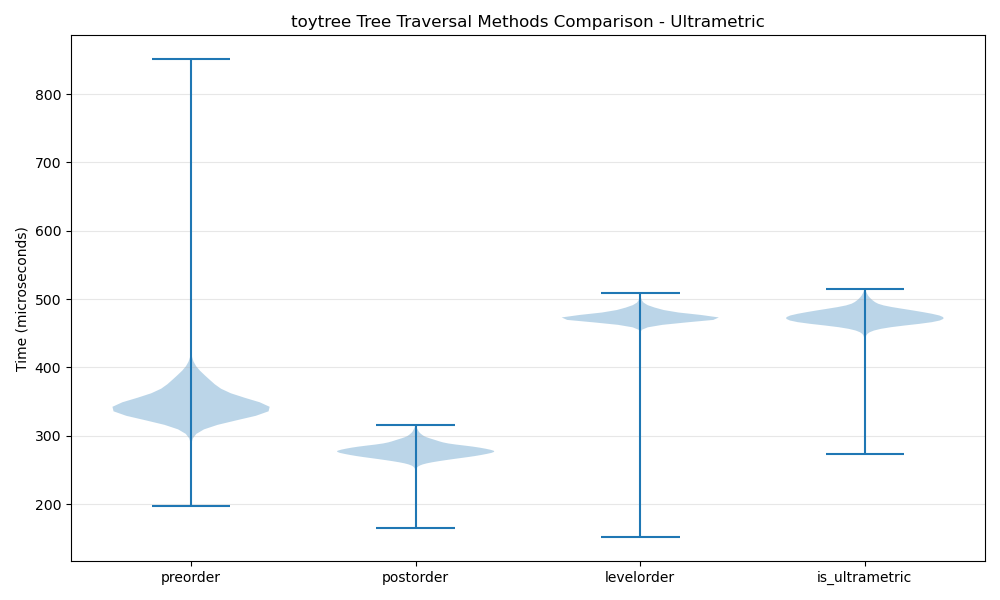
\includegraphics[width=\linewidth]{toytree_traverse_ultra.png}
        \caption{\toytree}
    \end{subfigure}
    \hfill
    \begin{subfigure}[b]{0.49\textwidth}
        
\includegraphics[width=\linewidth]{cogent3_traverse_ultra.png}
        \caption{\cogent}
    \end{subfigure}
    \caption{Traversal time distributions for \toytree\ (a) and \cogent\ (b) on the ultrametric tree set. Traversal strategies in order (left-to-right): pre-order, post-order, level-order, ultrametricity evaluation.}
    \label{fig:fast_python_traverse}
\end{figure}

\paragraph{Moderate Python Tools (\dendropy, \biopython, \ete)}

\pagebreak
\dendropy achieves moderate performance ($579-793\mu\text{s}$), acceptable for interactive workflows but slower than the two previous alternatives.
\ete has one the fastest pre-order traversal times ($238\mu s$), but has a comparatively slower post-order and level-order traversals ($>550\mu s)$.
Lastly, while excellent on ultrametricity checking
($435\mu\text{s}$),  \biopython\ is much slower on its built-in traversals ($\sim 3{,}250\mu\text{s}$) than the rest of the python-based tools (fig.\ref{fig:moderate_python_traverse}). 

\begin{figure}[htbp]
    \centering
    \begin{subfigure}[b]{0.3\textwidth}
        
\includegraphics[width=\linewidth]{dendropy_traverse_ultra.png}
        \caption{\dendropy}
    \end{subfigure}
    \hfill
    \begin{subfigure}[b]{0.3\textwidth}
        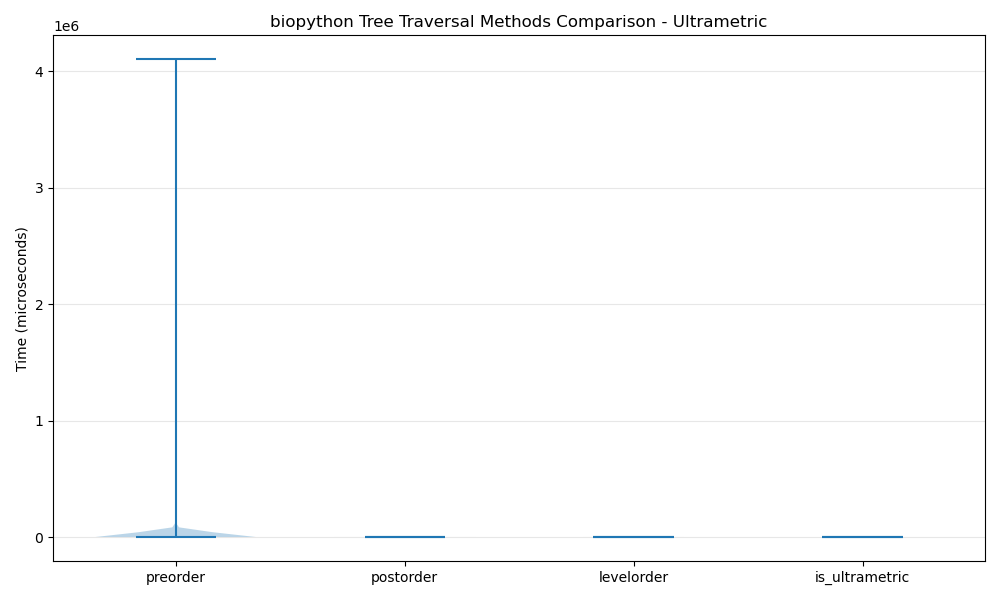
\includegraphics[width=\linewidth]{biopython_traverse_ultra.png}
        \caption{\biopython}
    \end{subfigure}
    \hfill
    \begin{subfigure}[b]{0.3\textwidth}
        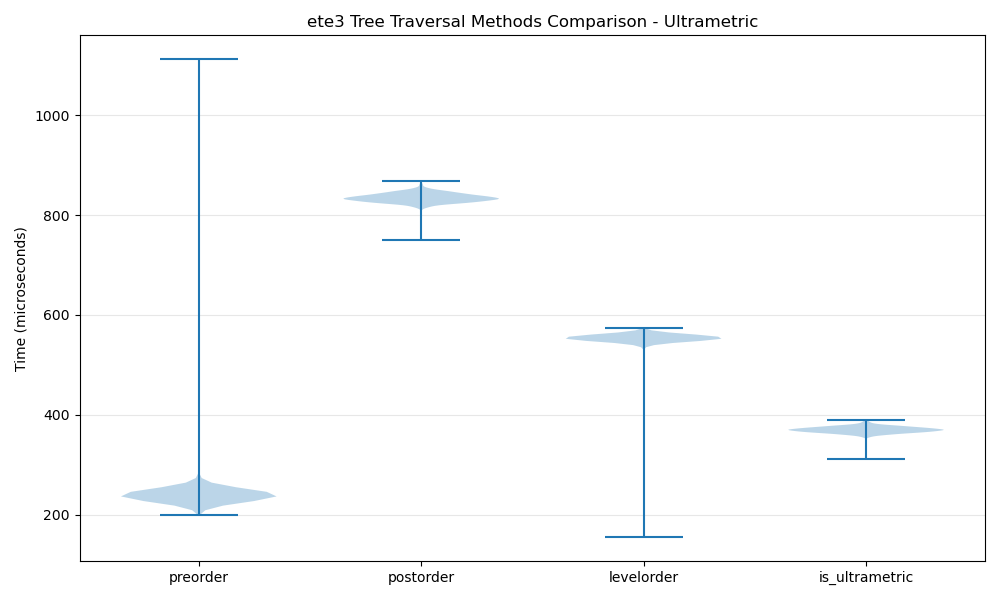
\includegraphics[width=\linewidth]{ete3_traverse_ultra.png}
        \caption{\ete}
    \end{subfigure}
    \caption{Traversal time distributions for \dendropy\ (a), \biopython\ (b) and \ete\ on the ultrametric tree set). Traversal strategies in order (left-to-right): pre-order, post-order, level-order, ultrametricity evaluation.}
    \label{fig:moderate_python_traverse}
\end{figure}

\paragraph{Julia (\phylo)}

\phylo\ demonstrates moderate traversal performance ($\sim750\mu\text{s}$
pre-order) with high variance, reflecting JIT compilation warm-up costs. The median times are comparable to moderately efficient python tools, but the high standard deviation ($\sim 13{,}097\,\mu\text{s}$ for pre-order) makes performance predictions unreliable (fig.\ref{fig:diverse_traverse}). By running its script several times, we confirmed that the maximum value was located on a different index each time (therefore, it was not a specific tree that caused such a significant variation). 

\begin{figure}[htbp]
    \centering
    \begin{subfigure}[b]{0.3\textwidth}
        
\includegraphics[width=\linewidth]{phylo_jl_traverse_ultra.png}
        \caption{\phylo}
    \end{subfigure}
    \hfill
    \begin{subfigure}[b]{0.3\textwidth}
        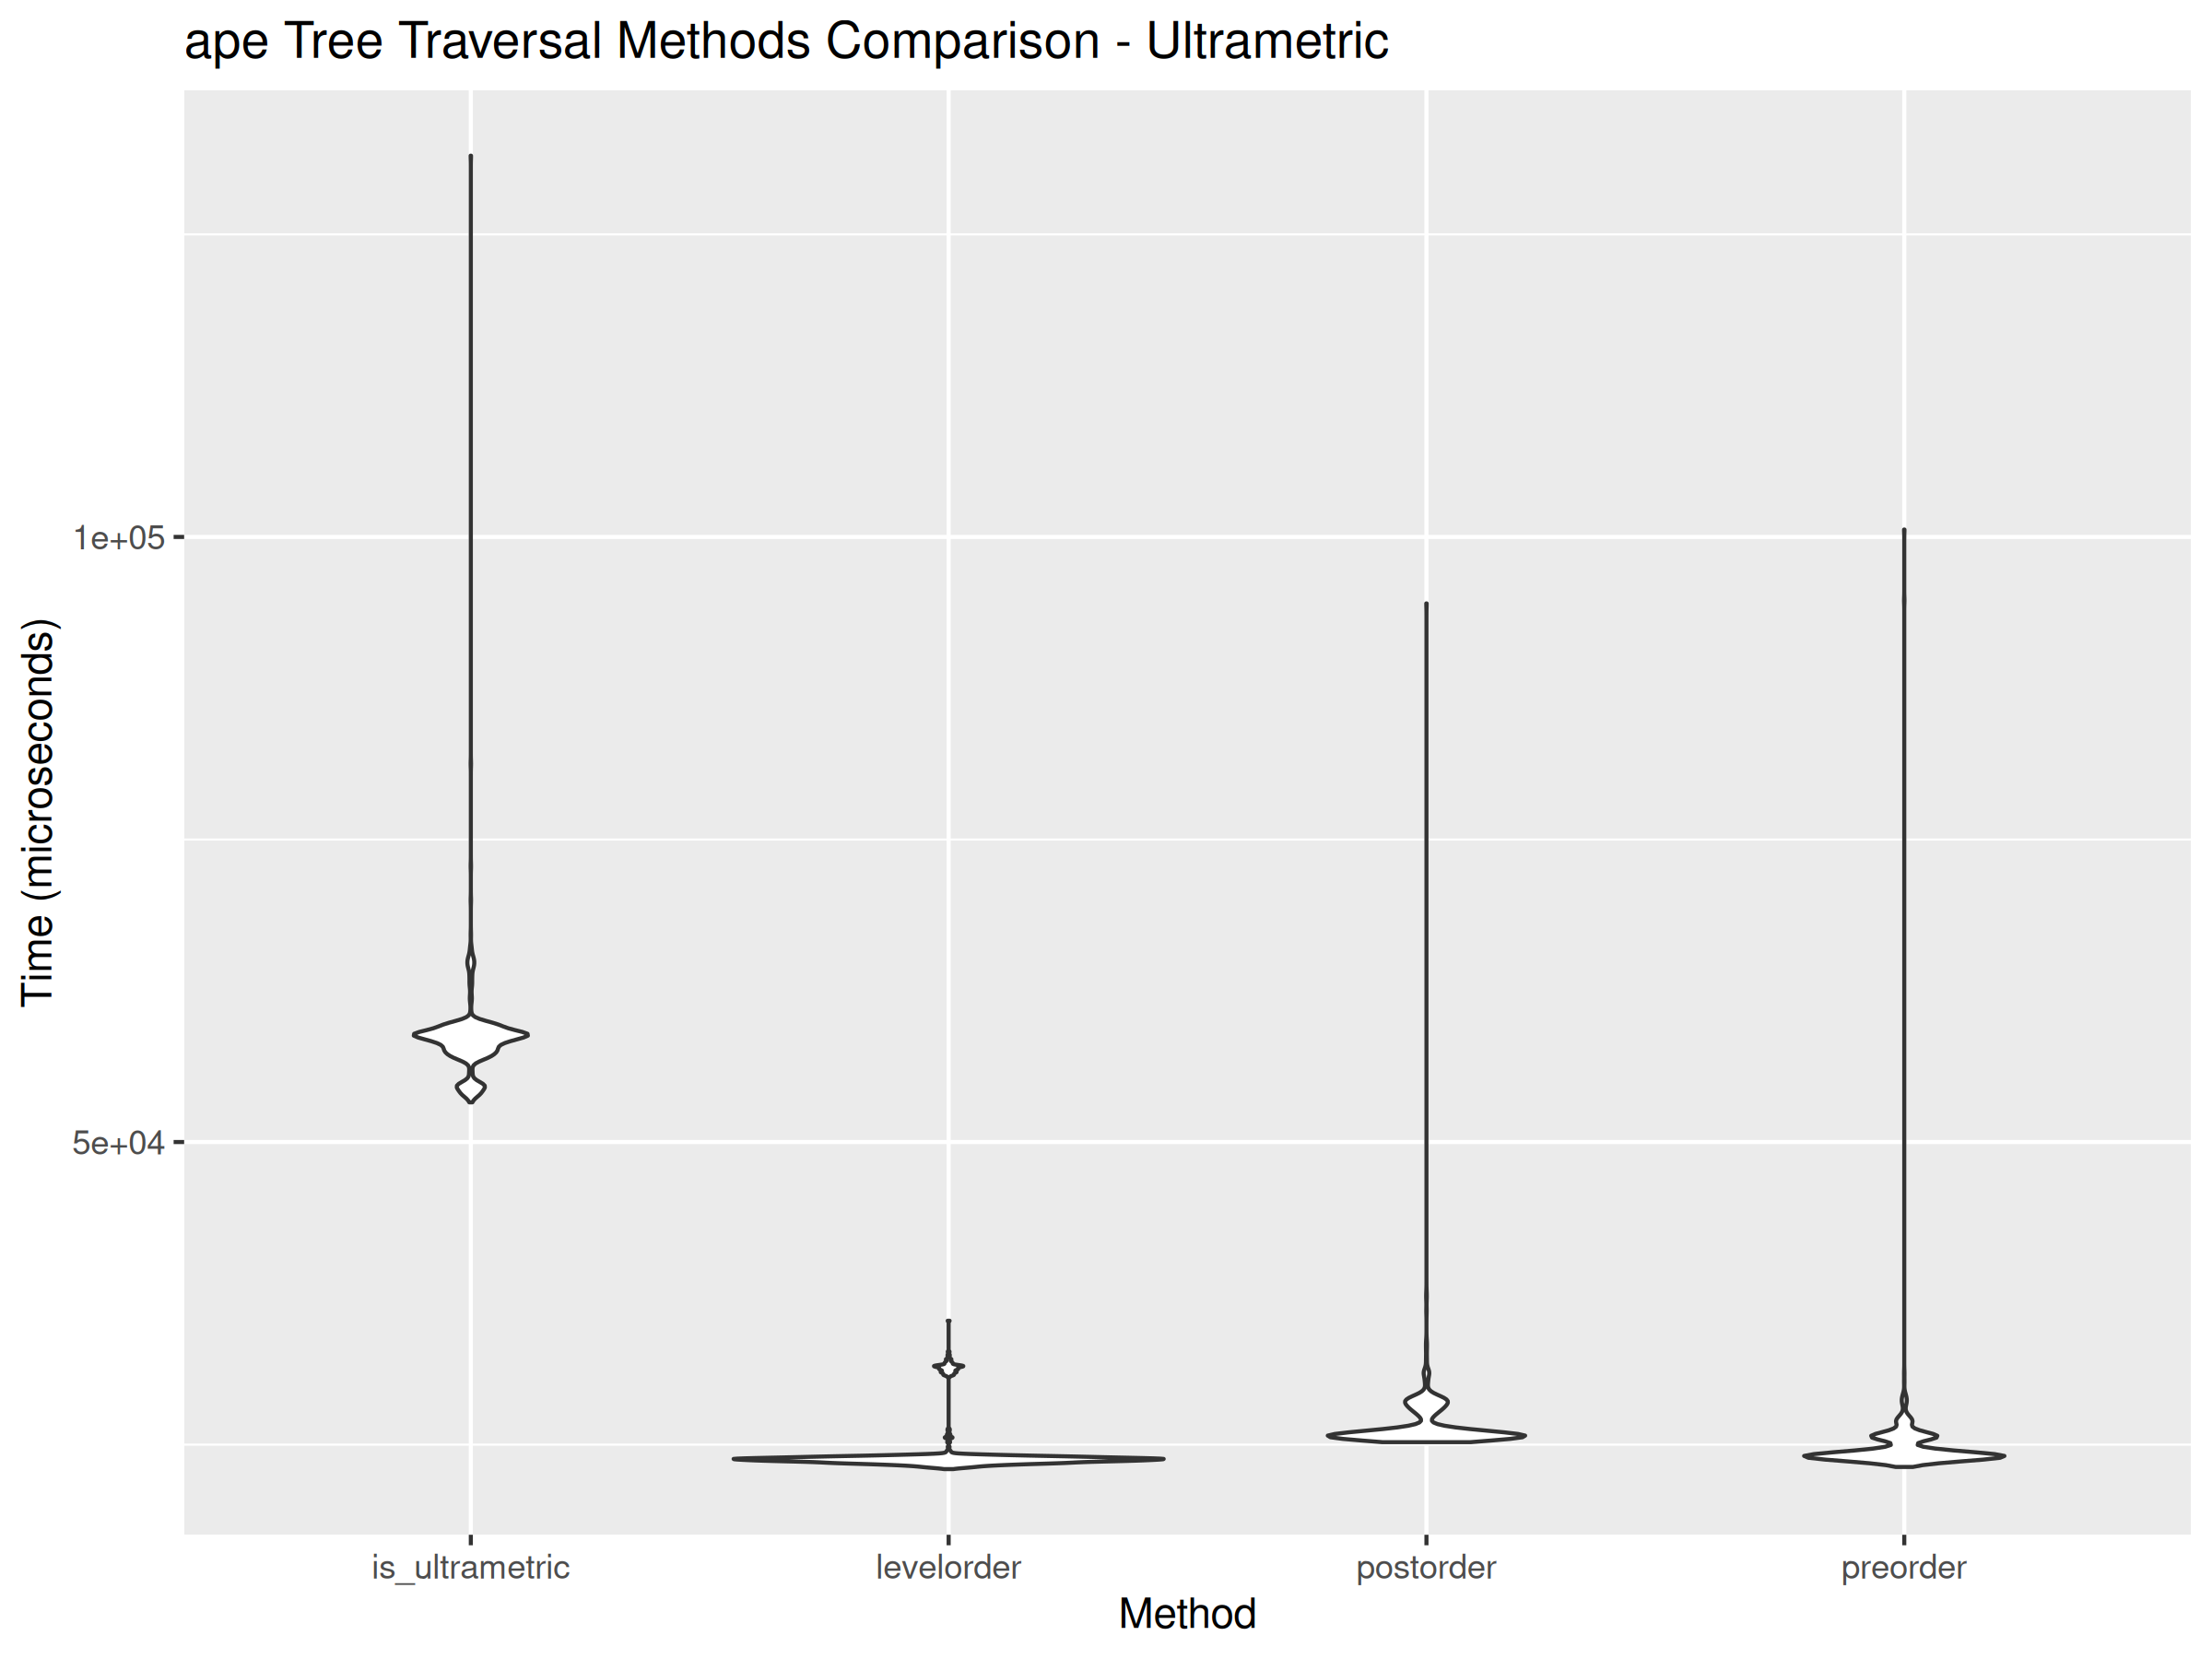
\includegraphics[width=\linewidth]{ape_traverse_ultra.png}
        \caption{\ape}
    \end{subfigure}
    \hfill
    \begin{subfigure}[b]{0.3\textwidth}
        
\includegraphics[width=\linewidth]{castor_traverse_ultra.png}
        \caption{\castor}
    \end{subfigure}
    \caption{Traversal time distributions for \phylo\ (a), \ape\ (b) and \castor\ on the ultrametric tree set). Traversal strategies in order (left-to-right): pre-order, post-order, level-order, ultrametricity evaluation.}
    \label{fig:diverse_traverse}
\end{figure}

\paragraph{R Tools (\ape, \castor)}

Both R packages are significantly slower than the rest of the tools. Among the two, \ape's median is two times that of \castor across all three strategies, whereas the ultrametric traversal has a smaller time difference. As the manually implemented traversal algorithms are the same for both, this difference most likely comes from \ape's \texttt{read.tree()} preserving the Newick traversal order of edges, while \castor's \texttt{read\_tree()} returns edges in pre-order order. Thus the parent column is already grouped for \castor, allowing \texttt{split()} to bucket children efficiently, whereas for \ape\ the parent column is not grouped and \texttt{split()} must build the groups from on every call. For this reason, \castor\ was selected over \ape for part II. 

\subsubsection{Tree Size Scaling}

Evaluation on larger trees (10{,}000 leaves) to assess algorithmic complexity and
scalability is pending. Expected asymptotic complexity is $O(n)$ for all traversal
methods; deviations would indicate implementation inefficiencies (e.g.\ quadratic
list operations).

% ------------------------------------------
\subsection{Coalescent Likelihood Evaluation}
% ------------------------------------------

\subsubsection{Tool and traversal strategy selection}

Based on the tree traversal benchmark results, the following tools were chosen: 
\begin{itemize}
    \item \toytree: Fastest Python tool; as it leans more on its visualization aspect, it would be interesting to note whether the performance is maintained on more complex frameworks
    \item \cogent: Fast Python tool; as it is part of a very diverse, Jupyter-compatible librairy, this tool is particularly interesting 
    \item \castor: Manual implementation of traversals resulted in higher performance than the other R-based tool, \ape. It will be chosen as a point of comparison and representative of the R language.
    \item \phylo: The only Julia tool studied, it generally produces medium times, but has an exceedingly high maximum value for post-order traversal which is worth looking further into.
\end{itemize}

Moreover, the tree traversal implemented in the interval extraction algorithm varied according to the better traversal strategy for each tool: pre-order traversal for \cogent\ and \castor, post-order traversal for \phylo\ and \toytree. 

\subsubsection{Interval extraction and log-likelihood performance}

Before implementing the entire coalescent likelihood framework, the interval extraction was benchmarked as a middle step. The summary results for both tests can be found in tab.\ref{tab:coal}, and the full output in the appendix. 

\begin{table}[h!]
\centering
\caption{Summary of tool performance for coalescent likelihood calculation.
         Median times in microseconds (1000-leaf heterochronic trees).}
\label{tab:coal}
\begin{tabular}{lcccc}
\toprule
\textbf{Tool} & \textbf{Language} & \textbf{Intervals} & \textbf{Log-likelihood} \\
\midrule
\cogent       & python    & 1{,}627     & 2{,}067  \\
\toytree     & python & 4{,}670 & 5{,}123 \\
\castor    & R & 6{,}953 & 7{,}514 \\
\phylo        & Julia     & 3{,}089 & 3{,}839 \\
\bottomrule
\end{tabular}
\end{table}
\paragraph{Python}

Surprisingly, \cogent\ was at least two times faster than \toytree\ for the coalescent likelihood functions; the latter of which has particularly high results when compared to simple traversal benchmarking. This reaffirms \cogent's potential, and is also a reminder that \toytree's main focus is visual and not computational.

\begin{figure}
    \centering
    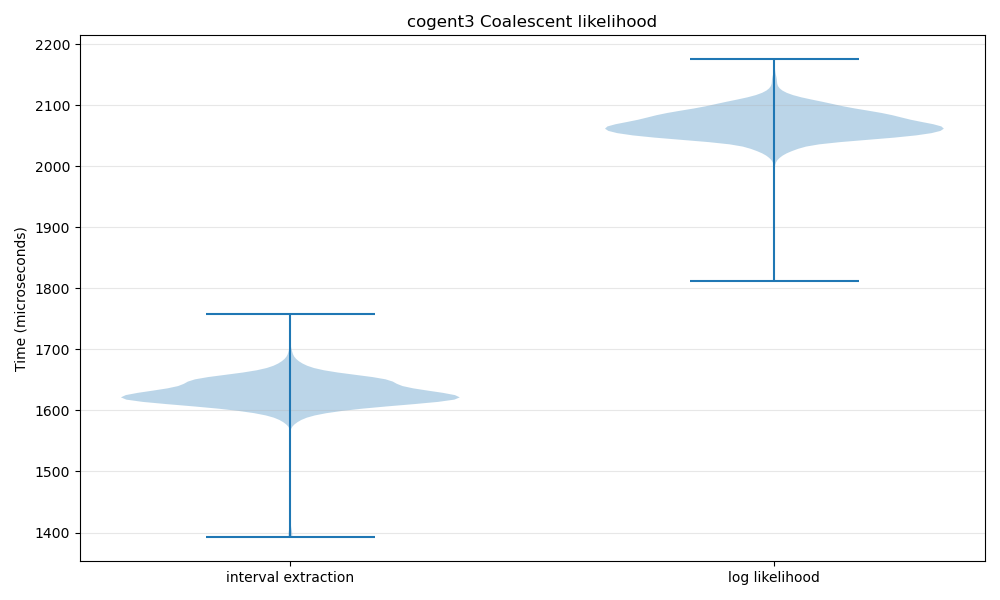
\includegraphics[width=0.4\linewidth]{cogent3_coal_lik.png}
    
\includegraphics[width=0.4\linewidth]{toytree_coal_lik.png}
    \caption{Interval extraction and coalescent likelihood calculation benchmark distributions in that order using \cogent (left) and \toytree (right).}
    \label{fig:cogent_coal}
\end{figure}

\paragraph{R}

\begin{figure}
    \centering
    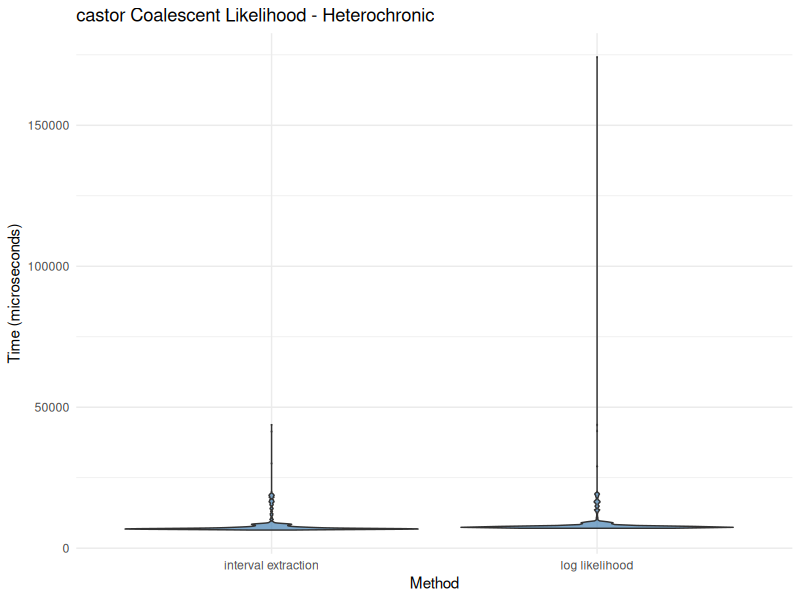
\includegraphics[width=0.4\linewidth]{castor_coal_likelihood_hetero.png}
    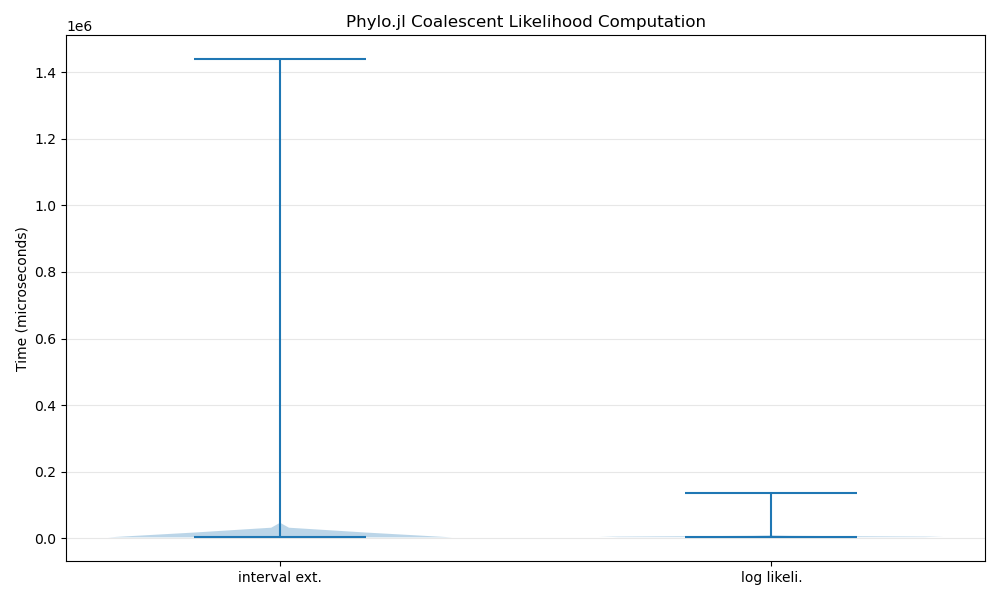
\includegraphics[width=0.4\linewidth]{phylo_jl_coal_likelihood.png}
    \caption{Interval extraction and coalescent likelihood calculation benchmark distributions in that order using \castor (left) and \phylo (right).}
    \label{fig:castor_coal}
\end{figure}

Similarly to tree traversal test, \castor\ appears to be slower than the other tools. This is what would be expected from an R tool. 

\paragraph{Julia}

Despite \phylo\ not being near the most efficient tools studied, the results based on Julia are better than some of the fast tools for simple traversals (tab.\ref{tab:coal}). This supports the claim that it's the \phylo\ package that is currently inefficient, and not Julia itself. The language would therefore be a viable option to  incorporate into a bigger phylogenetic framework. However, a deeper analysis of how its GC and compilation work would most likely be necessary, since it also shows a significantly higher maximum value for the interval extraction ($1.44 \times10^6 \mu s$; fig.\ref{fig:castor_coal}).

% ==========================================
% 4. CONCLUSIONS AND PERSPECTIVES
% ==========================================
\section{Conclusions and Perspectives}

\subsection{Key Findings}

The benchmarking exercise reveals performance differences of more than two orders of magnitude across eight tools, highlighting the importance of choosing the right phylogenetic library and the timing repercussion it has in downstream analyses. At one extreme, the high-performing Python tools, \cogent\ and \toytree, complete every traversal operation on a 1\,000‑leaf tree in under a half millisecond (Table~\ref{tab:summary}).  At the other extreme, \ape\ requires tens of milliseconds for the same operations, and its native
ultrametricity test approaches $60\,000\,\mu\text{s}$. The other R-based package, \castor, is faster than \ape\ but also remains an order of magnitude slower than the fastest Python libraries. This pattern confirms that a compiled backend, or at least a performance-focused implementation, is essential for performance‑critical tree manipulation.

However, language choice alone does not determine speed.  Within Python, \ete's preo-rder traversal is the single fastest measurement ($238\,\mu\text{s}$), while its post-order traversal is the slowest built-in Python measurement ($834\,\mu\texts$); \biopython\ is fast on the ultrametricity check but slow on general traversals. These variations across tools of the same language show that algorithmic details and data‑structure design are at least as important as the language itself.  \phylo\ illustrates the same point from the Julia side: Julia's
compilation model should, in principle, match or exceed the compiled Python tools, but the current \phylo\ implementation is only mid‑range and exhibits large variance, most likely because of JIT warm‑up or garbage collection.

The coalescent likelihood results reinforce the importance of the traversal backend.  \cogent\ evaluates the full exponential‑growth likelihood in about $2\,000\,\mu\text{s}$ per 1\,000‑leaf heterochronic tree, which is two to three times faster than \toytree, \phylo, and \castor\ (Table~\ref{tab:coal}).  Because likelihood evaluation decomposes into an interval‑extraction pass followed by a closed‑form sum, the cost of the underlying tree traversal sets a direct upper bound on inference input and output that would then go into MCMC or similar workflows.  Finally, although \phylo\ is not yet the fastest tool, Julia's broader inference ecosystem including \turing, and one of its associated packages, AdvancedHMC \cite{xu2020advancedhmc}; as well as the option to parallelize Julia scripts natively, makes it one of the most attractive platform for building a next‑generation, flexible phylogenetic inference toolkit. 

\subsection{Recommendations}

These results lead to the following practical guidance.  For interactive
exploration and high‑quality visualization, \ete\ and \toytree\ remain excellent choices: they are easy to script and their moderate runtimes are acceptable when trees are inspected one at a time. For
performance‑critical traversal or when many trees must be processed, the
optimized Python tools are clearly preferable, with \cogent\ offering the
most consistent performance and \dendropy\ providing a robust pure‑Python
fallback. For coalescent likelihood evaluation on the tested tree size,
\cogent\ is the fastest option; \castor\ should be used when an R workflow or ecosystem is required, and \ape\ should be reserved for tasks where its extensive native functionality outweighs raw speed.  Looking beyond these immediate benchmarks, the long‑term recommendation for complex phylogenetic inference is to invest in a Julia implementation: a single language that combines tree manipulation with automatic differentiation, HMC, particle filters, and neural posterior estimation would surpass the flexibility of current BEAST/BEAST2 XML pipelines. This could be achievable with Julia, despite its relatively smaller package diversity when compared to Python. 
\bigskip
\subsection{Future Directions}

Several extensions follow naturally from this work.  First, the most promising tools should be tested on bigger data sets (artificial 10\,000‑leaf tree sets have already been generated, another option would be real outbreak phylogenies), so that scaling behavior and memory usage can be characterized alongside raw CPU time.  Second, a more thorough investigation of Julia's warm‑up and garbage‑collection behaviour is needed, because the high variance seen in \phylo\ suggests that the language's theoretical speed is not yet fully realized by the current package.  Third, other demographic models, such as
the piecewise Skyline coalescent and the birth--death sampler model, should be added to the benchmarking framework, taking advantage of its modular design.  Fourth, it would be valuable to port selected BEAST models to Julia or Python, combining efficient tree operations with modern inference algorithms that are inaccessible inside BEAST's XML interface.  Fifth, once enough performance data is collected, frameworks combining different languages and packages could be used to optimize longer workflows, where the most efficient tool varies significantly across its tasks. Lastly, alternative tree encodings, including vector‑based representations such as Phylo2Vec \cite{penn2025phylo2vec}, should be benchmarked against Newick for both traversal and likelihood evaluation, since a more compact encoding could remove parsing and reordering bottlenecks.

% ==========================================
% REFERENCES
% ==========================================
\pagebreak

\section{References}

\begin{thebibliography}{99}

\bibitem{yang2012molecular}
Yang, Z., Rannala, B. (2012) Molecular phylogenetics: principles and practice. 
\textit{Nat Rev Genet} \textbf{13}, 303--314, nrg3186

\bibitem{whelan2001molecular}
Whelan, S., Liò, P., \& Goldman, N. (2001).
Molecular phylogenetics: state-of-the-art methods for looking into the past.
\textit{Trends in Genetics}, 17(5), 262--272.

\bibitem{ferreira2021covizu}
Ferreira, R.~C., Wong, E., Gugan, G., Wade, K., Liu, M., Baena, L.~M., Chato, C., Lu, B., Olabode, A.~S., \& Poon, A.~F.~Y. (2021).
CoVizu: Rapid analysis and visualization of the global diversity of SARS-CoV-2 genomes.
\textit{Virus Evolution}, 7(2), veab092.

\bibitem{volz2009}
Volz, E. M., et al. (2009).
Viral phylodynamics.
\textit{PLoS Computational Biology}, 5(3), e1000809.

\bibitem{pybus2001}
Pybus, O. G., et al. (2001).
Inferring the population size and growth history of HIV-1 from gene genealogies.
\textit{Journal of Virology}, 75(16), 7529--7539.

\bibitem{drummond2007beast}
Drummond, A. J., \& Rambaut, A. (2007).
BEAST: Bayesian evolutionary analysis by sampling trees.
\textit{BMC Evolutionary Biology}, 7, 214.

\bibitem{bouckaert2019beast2}
Bouckaert, R., Vaughan, T. G., Barido-Sottani, J., et al.\ (2019).
BEAST 2.5: An advanced software platform for Bayesian evolutionary analysis.
\textit{PLoS Computational Biology}, 15(4), e1006650.

\bibitem{carpenter2017stan}
Carpenter, B., Gelman, A., Hoffman, M. D., et al.\ (2017).
Stan: A probabilistic programming language.
\textit{Journal of Statistical Software}, 76(1), 1--32.

\bibitem{ge2018turing}
Ge, H., Xu, K., \& Ghahramani, Z. (2018).
Turing: A language for flexible probabilistic inference.
\textit{Proceedings of the 21st International Conference on Artificial Intelligence and Statistics (AISTATS)}, 84, 1682--1690.

\bibitem{salvatier2016pymc}
Salvatier, J., Wiecki, T. V., \& Fonnesbeck, C. (2016).
Probabilistic programming in Python using PyMC3.
\textit{PeerJ Computer Science}, 2, e55.

\bibitem{bezanson2017julia}
Bezanson, J., Edelman, A., Karpinski, S., \& Shah, V.~B. (2017).
Julia: A fresh approach to numerical computing.
\textit{SIAM Review}, 59(1), 65--98.

\bibitem{felsenstein1981evolutionary}
Felsenstein, J. (1981).
Evolutionary trees from DNA sequences: A maximum likelihood approach.
\textit{Journal of Molecular Evolution}, 17(6), 368--376.

\bibitem{hoehler2025phylosmew}
Höhler, D., Haag, J., Kozlov, A.~M., Morel, B., \& Stamatakis, A. (2025).
Performance assessment of phylogenetic inference tools using PhyloSmew.
\textit{Bioinformatics Advances}, 5(1), vbaf300.

\bibitem{paradis2004ape}
Paradis, E., Claude, J., \& Strimmer, K. (2004).
APE: analyses of phylogenetics and evolution in R language.
\textit{Bioinformatics}, 20(2), 289--290.

\bibitem{sukumaran2010dendropy}
Sukumaran, J., \& Holder, M.~T. (2010).
DendroPy: a Python library for phylogenetic computing.
\textit{Bioinformatics}, 26(12), 1569--1571.

\bibitem{berger2022scalene}
Berger, E.~D., Stern, S., \& Altmayer Pizzorno, J. (2022).
Triangulating Python performance issues with Scalene.
\textit{arXiv preprint} arXiv:2212.07597.

\bibitem{cogent32024}
Huttley, G., Maxwell, P., Caporaso, J.~G., \& contributors. (2024).
Cogent3: A toolkit for making sense from sequence.
GitHub repository. \url{https://github.com/cogent3/cogent3}

\bibitem{knight2007pycogent}
Knight, R., Maxwell, P., et al. (2007).
PyCogent: a toolkit for making sense from sequence.
\textit{Genome Biology}, 8(8), R171.

\bibitem{cock2009biopython}
Cock, P.~J.~A., et al.\ (2009).
Biopython: freely available Python tools for computational biology and
bioinformatics.
\textit{Bioinformatics}, 25(3), 422--423.

\bibitem{huerta2016ete3}
Huerta-Cepas, J., Serra, F., \& Bork, P. (2016).
ETE 3: reconstruction, analysis, and visualization of phylogenomic data.
\textit{Molecular Biology and Evolution}, 33(6), 1635--1638.

\bibitem{eaton2020toytree}
Eaton, D.~A. (2020).
toytree: A lightweight Python library for phylogenetics.
\textit{bioRxiv}.

\bibitem{phylojl2024}
White, G., et al. (2024).
Phylo.jl: A Julia package for phylogenetics.
GitHub repository. \url{https://github.com/JuliaPhylo/Phylo.jl}

\bibitem{kingman1982}
Kingman, J.~F.~C. (1982).
On the genealogy of large populations.
\textit{Journal of Applied Probability}, 19(A), 27--43.

\begin{comment}
\bibitem{griffiths1994}
Griffiths, R.~C., \& Tavar\'{e}, S. (1994).
Sampling theory for neutral alleles in a varying environment.
\textit{Philosophical Transactions of the Royal Society B}, 344, 403--410.
\end{comment}

\bibitem{teufel2018castor}
Louca, S., \& Doebeli, M. (2018).
Efficient comparative phylogenetics on large trees.
\textit{Bioinformatics}, 34(6), 1053--1055.

\bibitem{drummond2002}
Drummond, A.~J., Nicholls, G.~K., Rodrigo, A.~G., \& Solomon, W. (2002).
Estimating mutation parameters, population history and genealogy simultaneously from temporally spaced sequence data.
\textit{Genetics}, 161(3), 1307--1320.

\bibitem{xu2020advancedhmc}
Xu, K., Ge, H., Tebbutt, W., Tarek, M., Trapp, M., \& Ghahramani, Z. (2020).
AdvancedHMC.jl: A robust, modular and efficient implementation of advanced HMC algorithms.
In Zhang, C., Ruiz, F., Bui, T., Dieng, A.~B., \& Liang, D.\ (Eds.),
\textit{Proceedings of The 2nd Symposium on Advances in Approximate Bayesian Inference}
(pp.\ 1--10).

\bibitem{penn2025phylo2vec}
Penn, M.~J., Scheidwasser, N., Khurana, M.~P., Duch\^ene, D.~A., Donnelly, C.~A., \& Bhatt, S. (2025).
Phylo2Vec: A vector representation for binary trees.
\textit{Systematic Biology}, 74(2), 250--266.

\end{thebibliography}

\newpage

% ==========================================
% APPENDIX
% ==========================================
\section{Appendix}

\appendix

\section{Specifications}

\subsection{System Specifications}
\begin{itemize}
    \item OS: Linux Mint 22.3 x86\_64, 6.8.0-111-generic 
    \item Host: OMEN Gaming Laptop 16-ap0xxx 
    \item CPU: AMD Ryzen 9 8940HX with Radeon Graphics (32) @ 5.385GHz 
    \item GPU: AMD ATI 07:00.0 Raphael, NVIDIA 01:00.0 NVIDIA Corporation Device 2d19 
    \item RAM: 32 GB
\end{itemize}

\subsection{Tool Specifications}

\begin{itemize}
    \item \ape: Version 5.8.1; R 4.x, C/C++ backend
    \item \castor: Version 1.8.5; R 4.x, C++ backend
    \item \dendropy: Version 5.0.8; Python 3.x
    \item \cogent: Version 2026.5.19a0; Python 3.x
    \item \biopython: Version 1.87; Python 3.x
    \item \ete: Version 3.1.3; Python 3.x
    \item \toytree: Version 3.0.11; Python 3.x
    \item \phylo: Version 0.5.4; Julia 1.x, LLVM JIT compilation
\end{itemize}

\subsection{Scripts}
The scripts for tree traversal (trav/traverse\_*.*) and coalescent likelihood (coal/coall\_*.*) are available on the project's github page: \url{https://github.com/cuajiniquil/internship26}.

\section{Detailed Results}

\subsection{Tree traversal benchmarking results}

\verbatiminput{res\_traverse.txt}

\subsection{Coalescent likelihood benchmarking results}

\verbatiminput{testres2.txt}
\end{document}